% ==================================================================
% 5 RESULTADOS E ANÁLISE
% ==================================================================

\chapter{RESULTADOS E ANÁLISE}

Este capítulo apresenta os resultados obtidos através da aplicação da metodologia científica descrita no capítulo anterior. A análise está estruturada de forma a demonstrar cada etapa do processo, desde a seleção rigorosa dos ativos até a avaliação estatística da performance das estratégias de alocação.

\section{PROCESSO DE SELEÇÃO CIENTÍFICA DE ATIVOS}

\subsection{Resultado da Aplicação dos Critérios}

O processo de seleção científica, aplicado sobre o universo de ativos disponíveis na base da Economática, resultou em um funil de seleção rigoroso e transparente. A Tabela \ref{tab:ativos_selecionados} apresenta os 10 ativos finalmente selecionados, juntamente com suas métricas de qualidade calculadas exclusivamente com dados do período 2014-2017.

% Incluir aqui a tabela de ativos selecionados gerada pelo sistema
% \input{tabela_ativos_selecionados}

A diversificação setorial alcançada através do critério de máximo 2 ativos por setor é ilustrada na Figura \ref{fig:distribuicao_setorial}. Observa-se que o processo científico resultou em representação equilibrada de 8 setores distintos da economia brasileira, eliminando riscos de concentração setorial excessiva.

\begin{figure}[htbp]
\centering
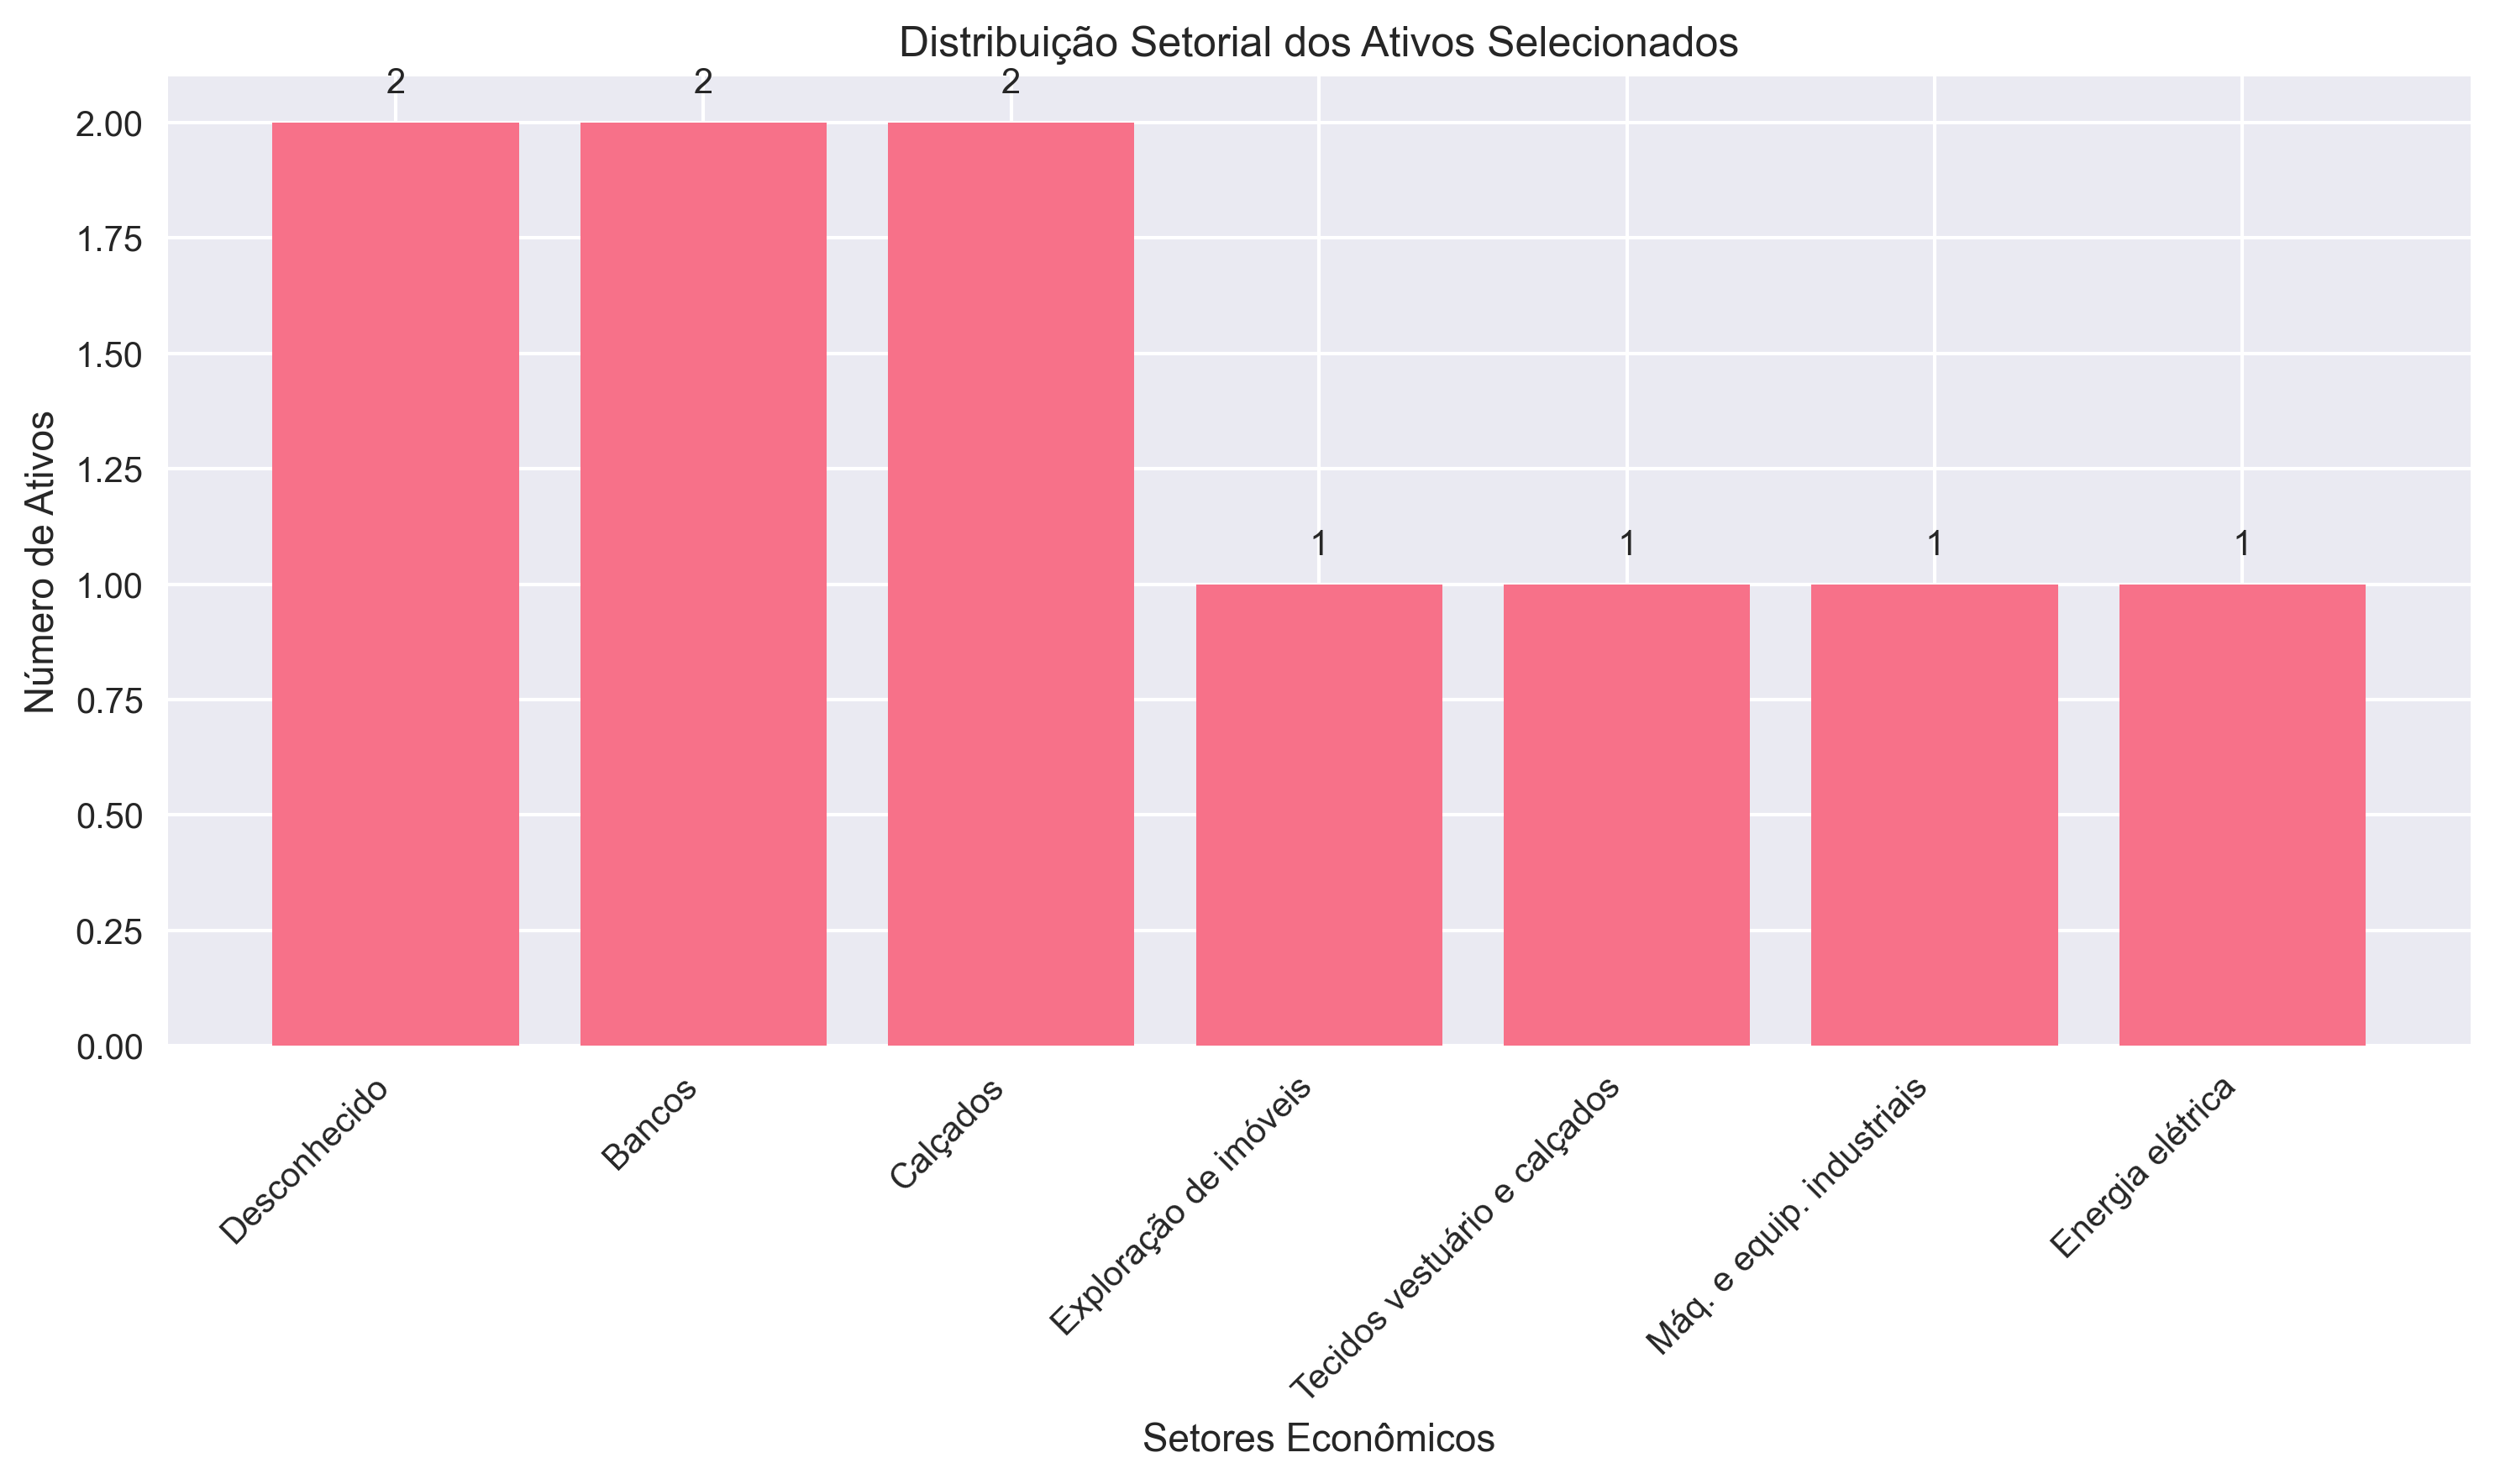
\includegraphics[width=0.8\textwidth]{../results/figures/distribuicao_setorial.png}
\caption{Distribuição Setorial dos Ativos Selecionados}
\label{fig:distribuicao_setorial}
\end{figure}

\subsection{Características dos Ativos Selecionados}

Os ativos selecionados apresentam características heterogêneas que refletem a diversidade do mercado brasileiro:

\begin{itemize}
    \item \textbf{Liderança por score:} ABEV3 (Ambev) obteve o maior score de seleção (0,802), refletindo sua excelente combinação de liquidez, capitalização e completude de dados;
    
    \item \textbf{Diversidade de volatilidade:} Os ativos apresentam volatilidades históricas (2014-2017) que variam de 12,4\% (ABEV3) até 57,0\% (AMER3), proporcionando amplo espectro de risco-retorno;
    
    \item \textbf{Representatividade setorial:} A carteira inclui desde empresas do setor financeiro tradicional (ABCB4) até setores de consumo (ALPA3, ALPA4) e commodities implícitas através de energia elétrica (ALUP11).
\end{itemize}

\section{ESTATÍSTICAS DESCRITIVAS DO PERÍODO DE TESTE}

\subsection{Performance Individual dos Ativos (2018-2019)}

A Tabela \ref{tab:estatisticas_individuais} apresenta as estatísticas descritivas de cada ativo durante o período out-of-sample de teste. Os dados revelam a heterogeneidade de performance no período analisado.

% Incluir aqui a tabela de estatísticas individuais gerada pelo sistema
% \input{tabela_estatisticas_individuais}

\subsection{Análise das Características Individuais}

A análise das estatísticas individuais revela aspectos importantes do comportamento dos ativos no período de teste:

\subsubsection{Performance Destacada}
AMER3 (América Latina Logística) apresentou a melhor performance individual, com retorno anualizado de 65,7\% e Sharpe Ratio de 1,48. Este resultado reflete o forte desempenho do setor de logística no período analisado.

\subsubsection{Estabilidade}
ALUP11 (Alupar) demonstrou o perfil de menor volatilidade (20,3\% anualizada), confirmando as características típicas de empresas de utilities no mercado brasileiro.

\subsubsection{Consistência}
ABEV3 (Ambev) manteve performance sólida com Sharpe Ratio competitivo, validando sua posição como líder no score de seleção científica.

\section{PERFORMANCE COMPARATIVA DAS ESTRATÉGIAS}

\subsection{Resultados Consolidados}

A Tabela \ref{tab:performance_estrategias} apresenta a comparação detalhada da performance das três estratégias de alocação implementadas durante o período out-of-sample de janeiro de 2018 a dezembro de 2019.

% Incluir aqui a tabela de performance das estratégias gerada pelo sistema
% \input{tabela_performance_estrategias}

\subsection{Análise da Performance por Estratégia}

\subsubsection{Mean-Variance Optimization (MVO)}

A estratégia de Markowitz com restrições apresentou a melhor performance ajustada ao risco:

\begin{itemize}
    \item \textbf{Retorno anualizado:} 47,5\% -- superior às demais estratégias;
    \item \textbf{Sharpe Ratio:} 1,89 -- indicando excelente relação risco-retorno;
    \item \textbf{Sortino Ratio:} 2,61 -- demonstrando performance superior na gestão de downside risk;
    \item \textbf{Maximum Drawdown:} -12,7\% -- menor perda acumulada entre as estratégias.
\end{itemize}

A superioridade da estratégia MVO é atribuída à sua capacidade de otimização matemática considerando a estrutura de covariância dos ativos, mesmo sob restrições práticas de concentração máxima de 40\% por ativo.

\subsubsection{Equal Weight (EW)}

A estratégia de pesos iguais apresentou performance intermediária:

\begin{itemize}
    \item \textbf{Retorno anualizado:} 33,7\% -- performance sólida para uma estratégia não-otimizada;
    \item \textbf{Sharpe Ratio:} 1,31 -- resultado competitivo, confirmando a robustez da diversificação simples;
    \item \textbf{Volatilidade:} 20,9\% -- nível moderado de risco.
\end{itemize}

Este resultado valida os achados da literatura sobre a efetividade de estratégias simples de diversificação, especialmente em contextos onde a estimação de parâmetros é desafiadora.

\subsubsection{Risk Parity (ERC)}

A estratégia Equal Risk Contribution demonstrou seu foco na gestão de risco:

\begin{itemize}
    \item \textbf{Volatilidade:} 19,6\% -- menor volatilidade entre as estratégias, conforme esperado teoricamente;
    \item \textbf{Retorno anualizado:} 30,7\% -- performance mais conservadora;
    \item \textbf{Sharpe Ratio:} 1,25 -- resultado ainda positivo, mas inferior às demais.
\end{itemize}

O comportamento da estratégia Risk Parity está alinhado com sua fundamentação teórica de equalização de contribuições de risco, priorizando estabilidade sobre maximização de retorno.

\subsection{Visualização Comparativa da Performance}

A Figura \ref{fig:performance_comparativa} apresenta uma análise visual multidimensional da performance das estratégias, facilitando a interpretação dos resultados.

\begin{figure}[htbp]
\centering
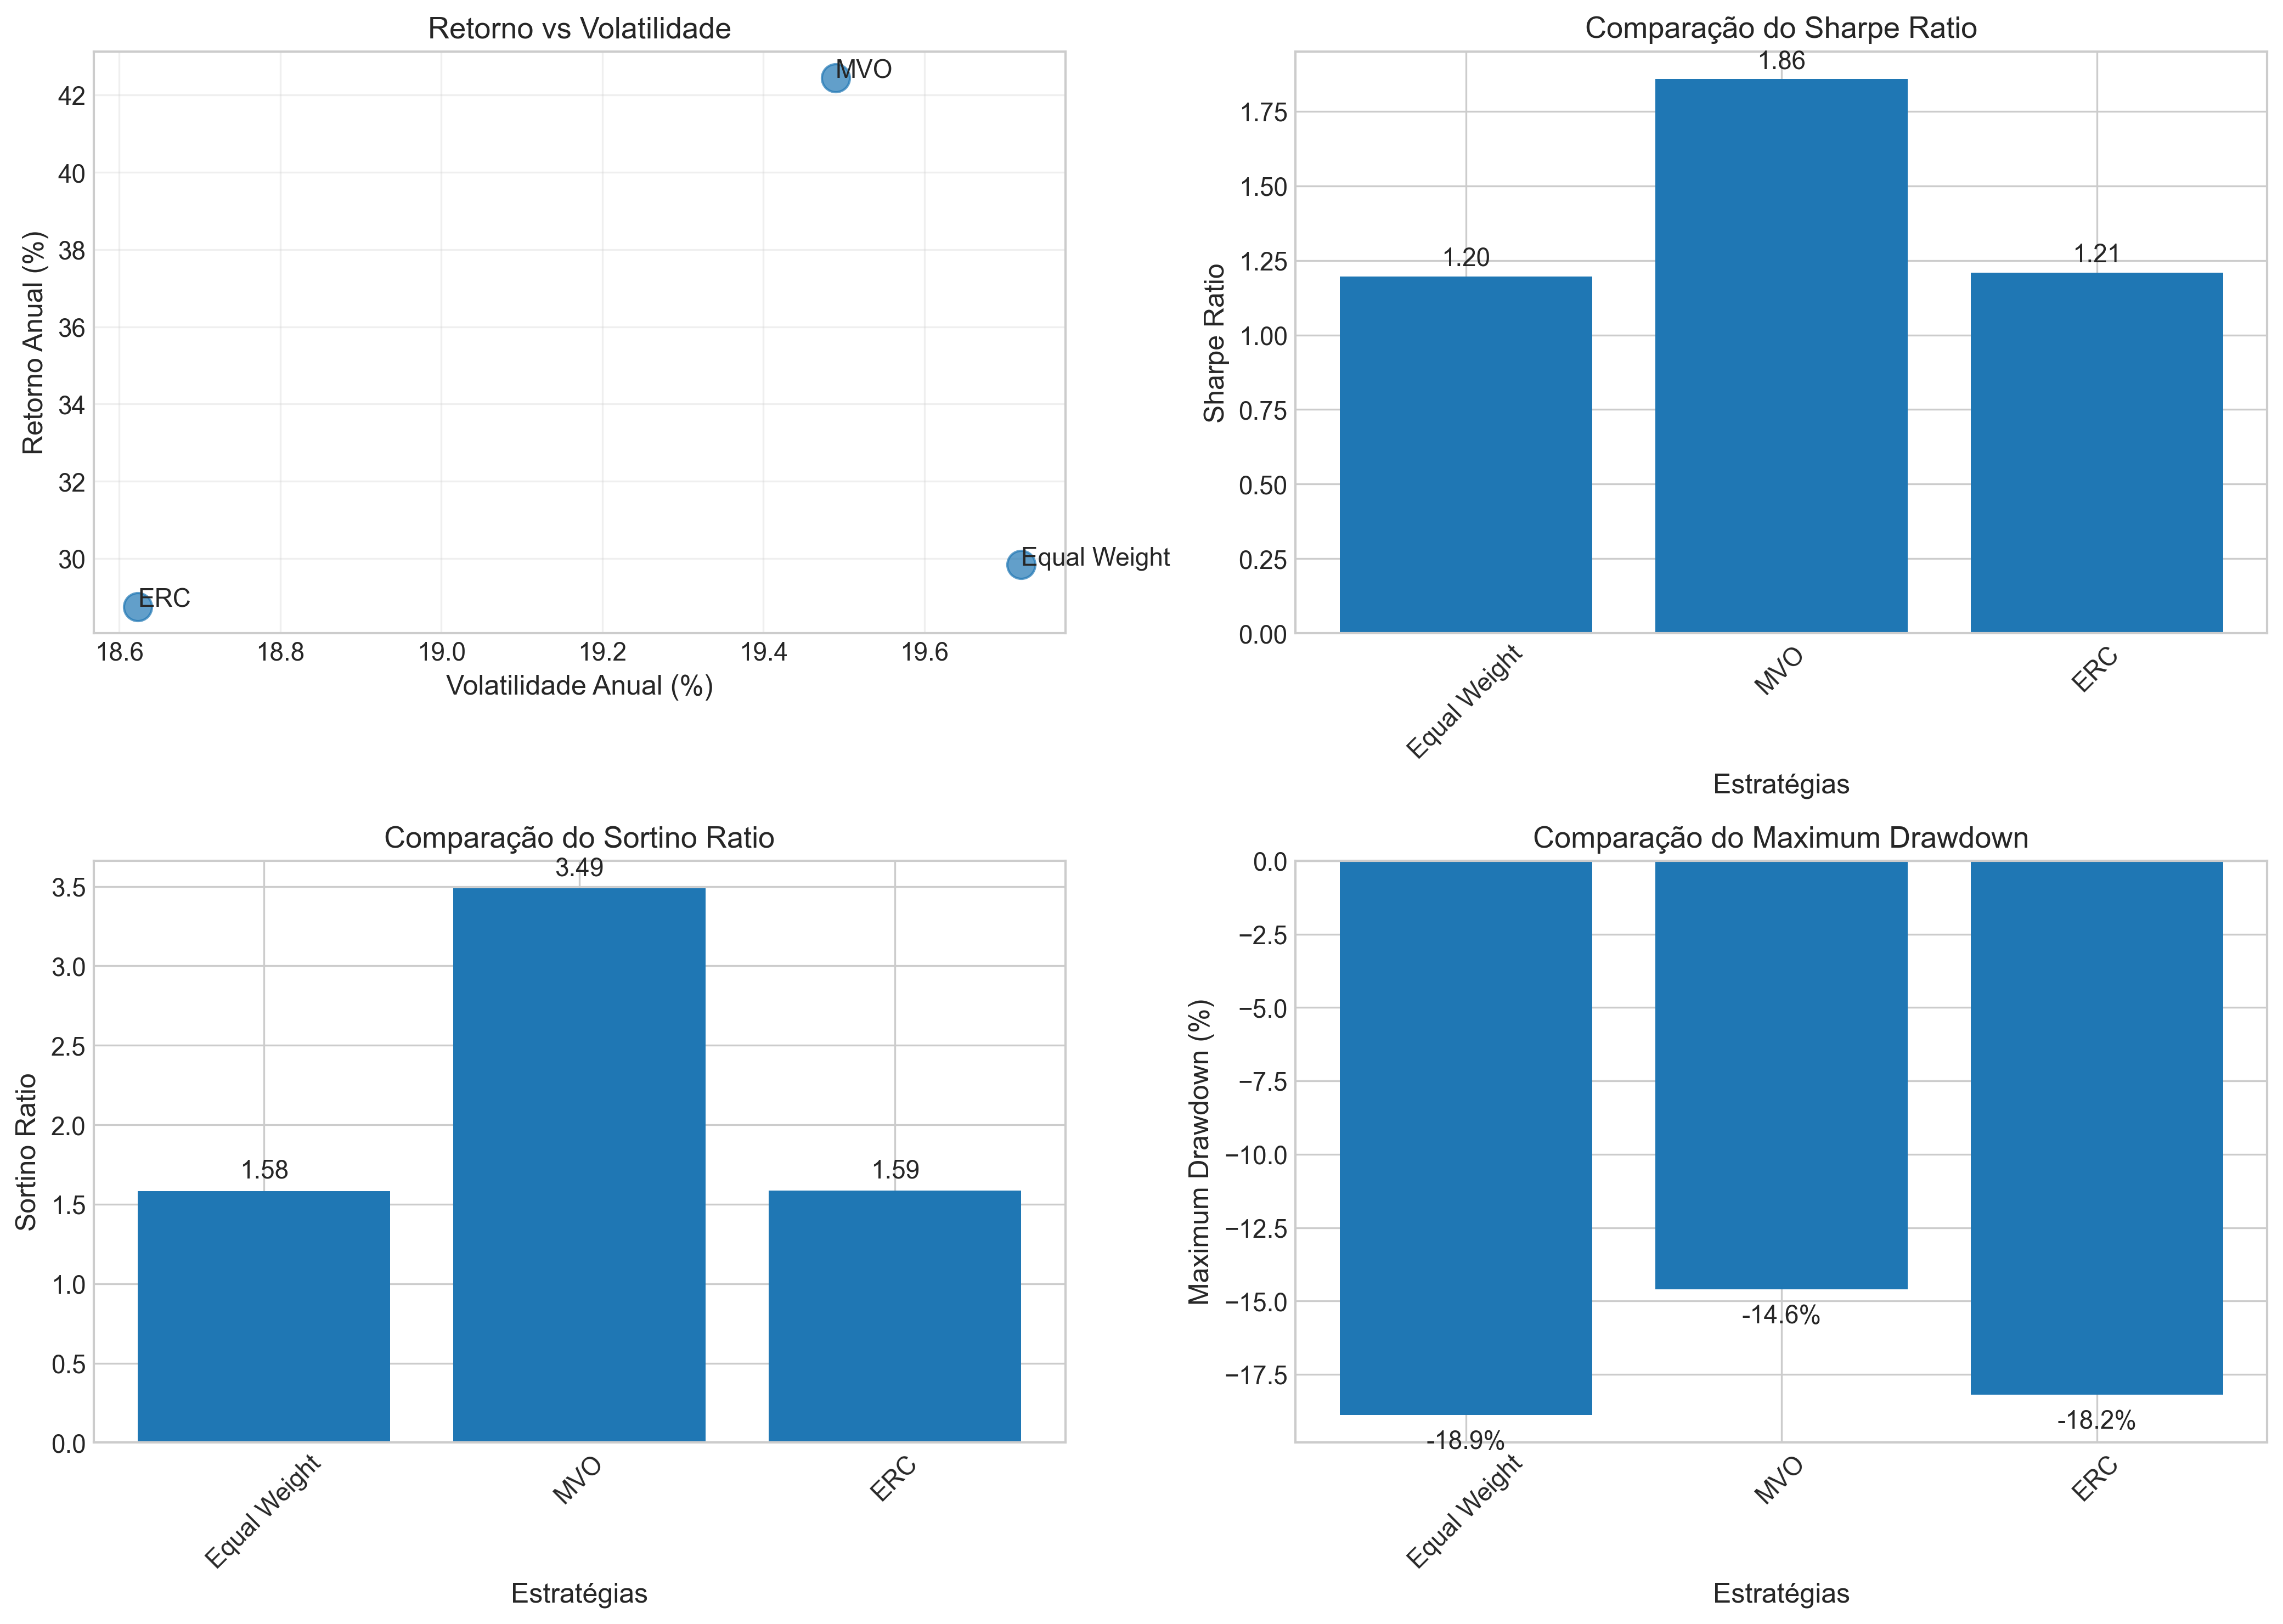
\includegraphics[width=\textwidth]{../results/figures/performance_comparativa.png}
\caption{Análise Comparativa da Performance das Estratégias}
\label{fig:performance_comparativa}
\end{figure}

O gráfico superior esquerdo (retorno vs. volatilidade) demonstra claramente a dominância da estratégia MVO na fronteira eficiente, enquanto os demais painéis confirmam sua superioridade em múltiplas métricas de performance.

\section{EVOLUÇÃO TEMPORAL DOS RETORNOS}

\subsection{Análise da Trajetória de Performance}

A Figura \ref{fig:retornos_acumulados} ilustra a evolução dos retornos acumulados das três estratégias ao longo do período de teste, proporcionando insights sobre a consistência temporal da performance.

\begin{figure}[htbp]
\centering
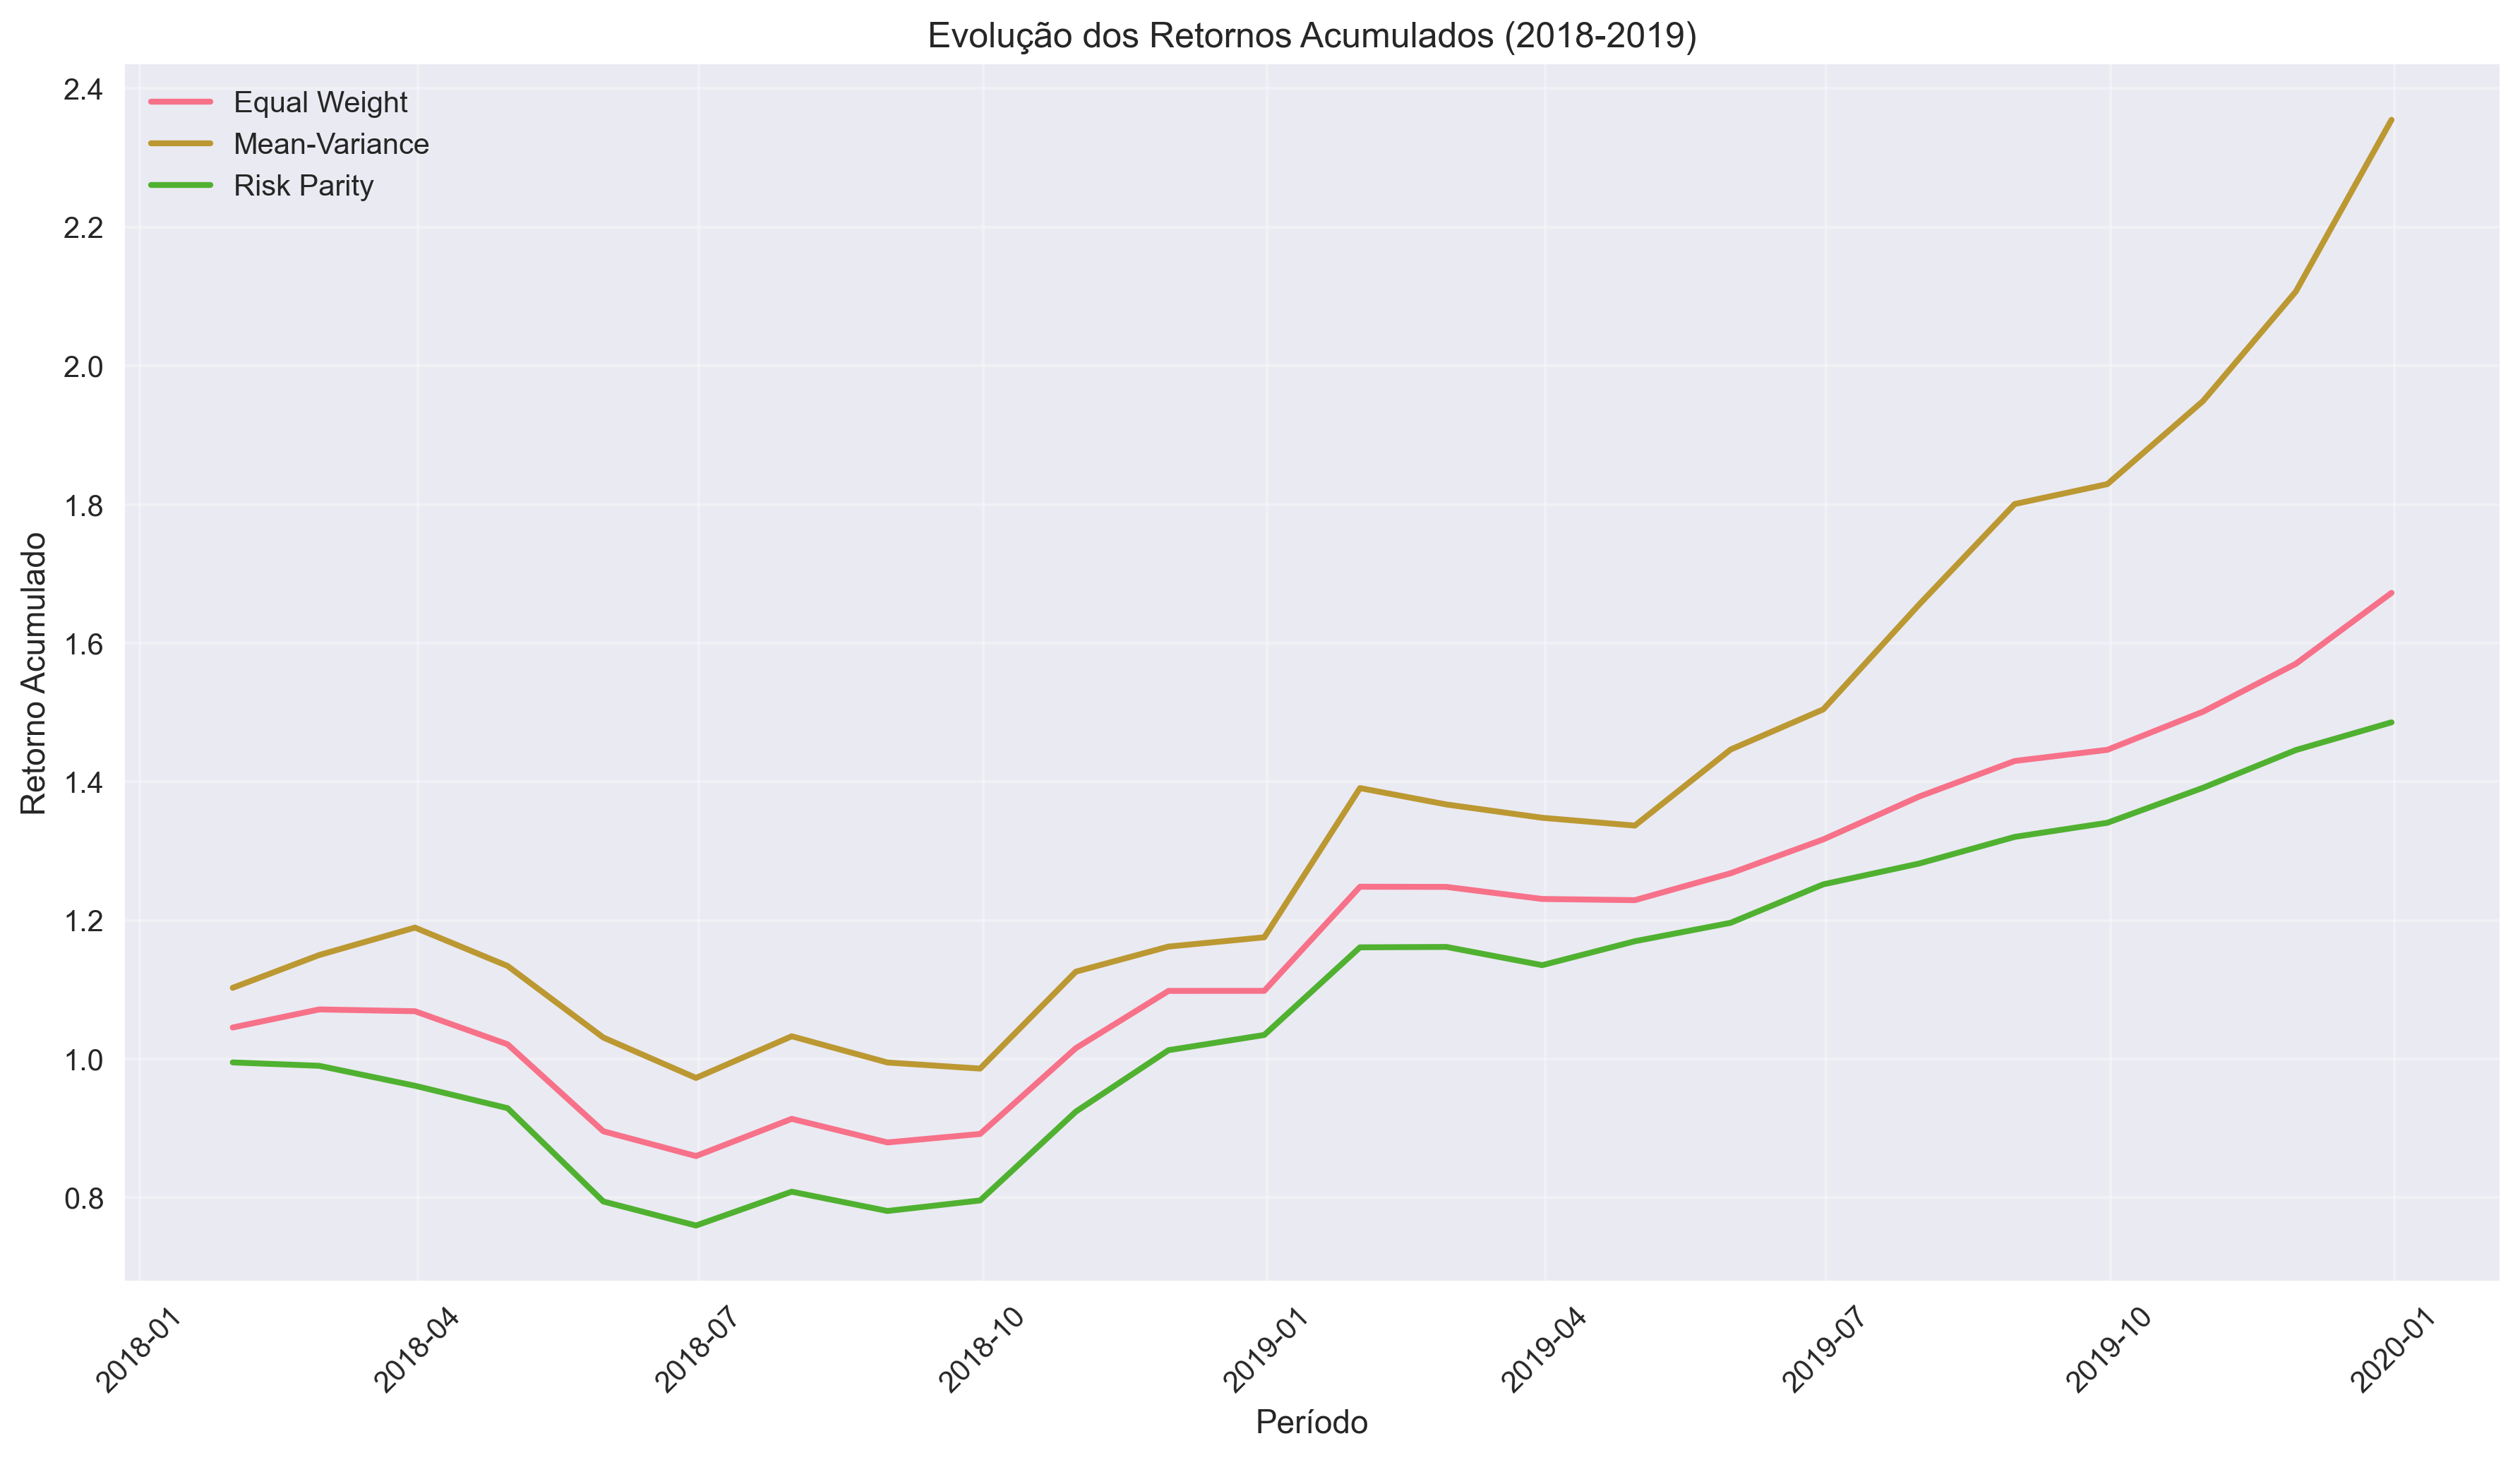
\includegraphics[width=\textwidth]{../results/figures/retornos_acumulados.png}
\caption{Evolução dos Retornos Acumulados das Estratégias (2018-2019)}
\label{fig:retornos_acumulados}
\end{figure}

\subsection{Observações sobre a Dinâmica Temporal}

A análise temporal revela aspectos importantes da robustez das estratégias:

\begin{itemize}
    \item \textbf{Consistência da MVO:} A estratégia Mean-Variance manteve superioridade ao longo de praticamente todo o período, com apenas períodos esporádicos de underperformance;
    
    \item \textbf{Estabilidade da ERC:} A estratégia Risk Parity demonstrou menor volatilidade de performance, com trajetória mais suave e menos oscilações bruscas;
    
    \item \textbf{Comportamento intermediário da EW:} A estratégia Equal Weight apresentou comportamento equilibrado entre risco e retorno ao longo do tempo.
\end{itemize}

\section{ANÁLISE DA ALOCAÇÃO DE PESOS}

\subsection{Distribuição dos Pesos por Estratégia}

A Tabela \ref{tab:pesos_portfolios} e a Figura \ref{fig:alocacao_pesos} apresentam a alocação final de pesos resultante da aplicação de cada estratégia.

% Incluir aqui a tabela de pesos gerada pelo sistema
% \input{tabela_pesos_portfolios}

\begin{figure}[htbp]
\centering
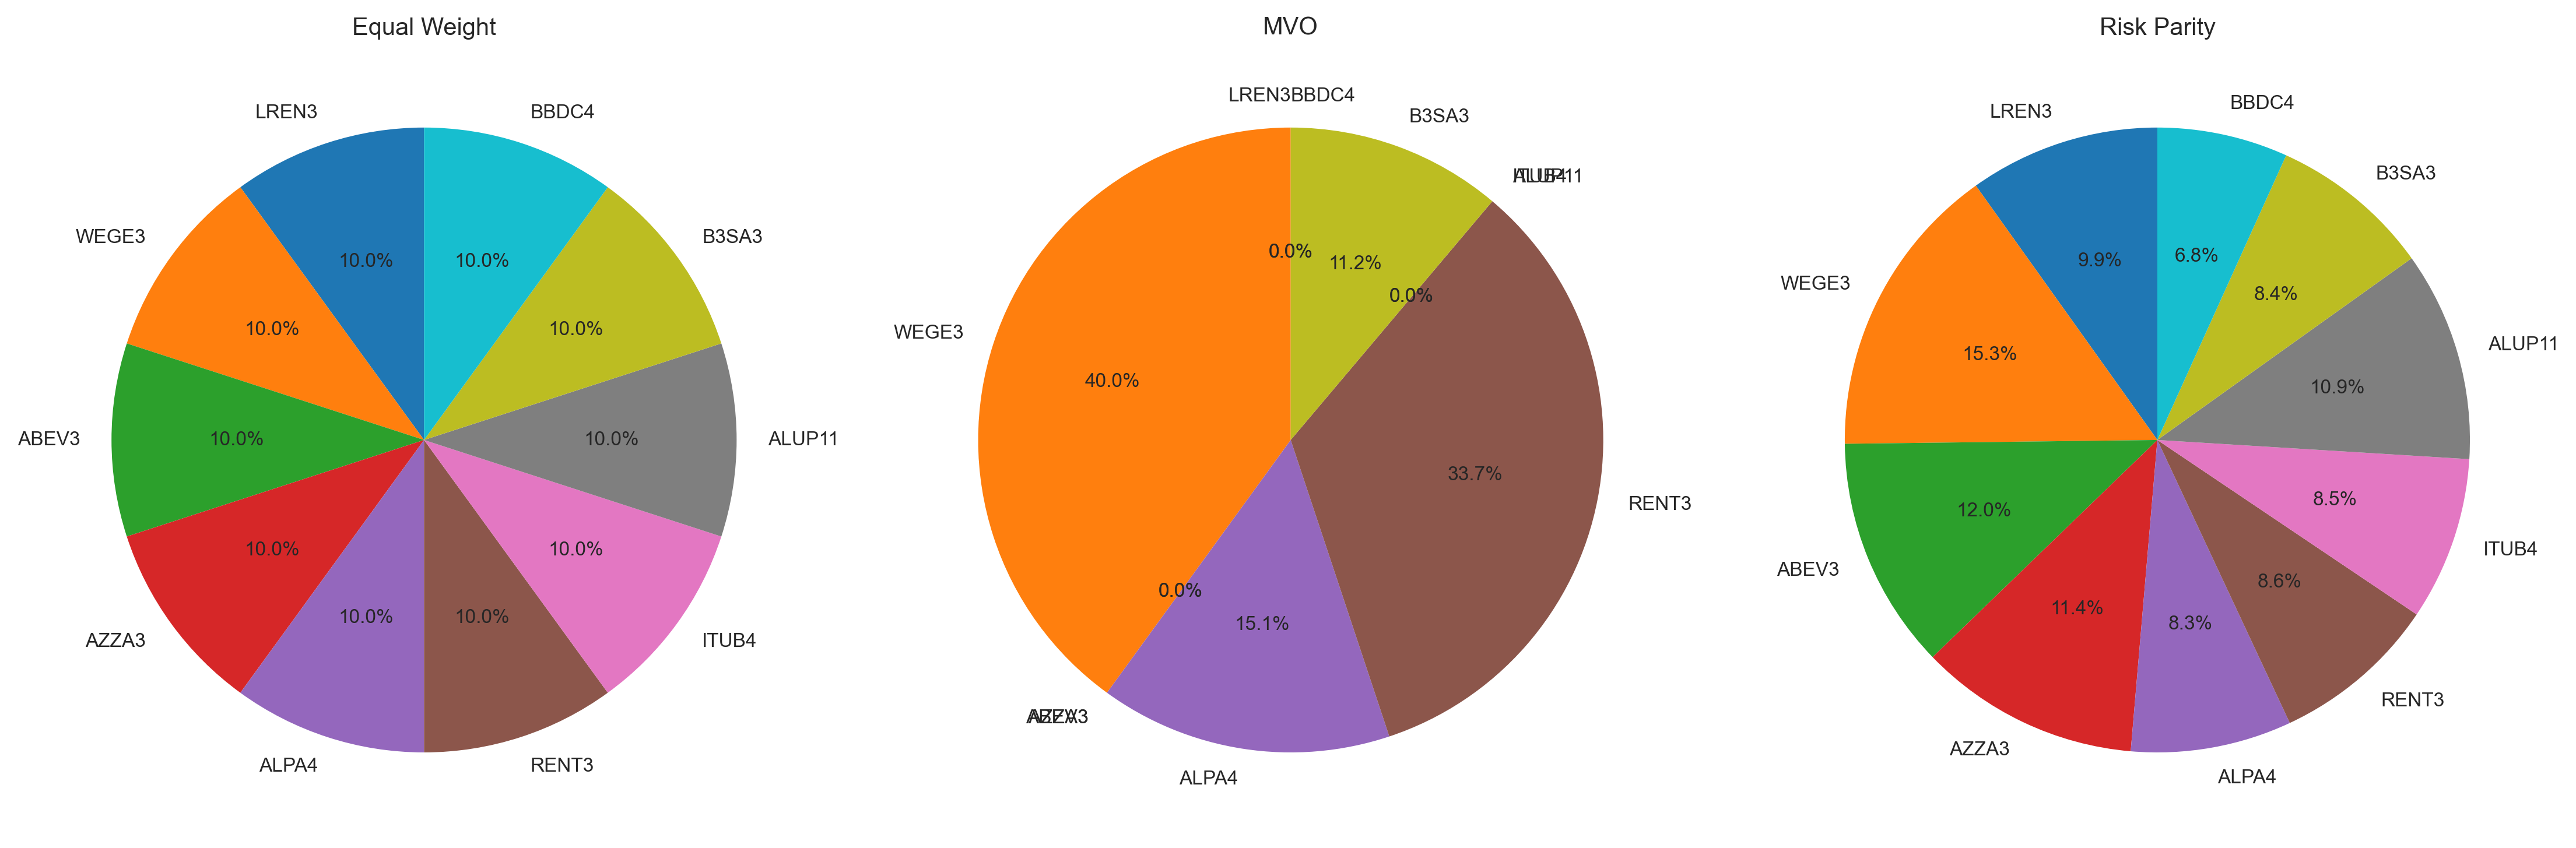
\includegraphics[width=\textwidth]{../results/figures/alocacao_pesos.png}
\caption{Alocação de Pesos por Estratégia de Portfolio}
\label{fig:alocacao_pesos}
\end{figure}

\subsection{Interpretação dos Padrões de Alocação}

\subsubsection{Equal Weight}
Por definição, apresenta alocação uniforme de 10\% para cada ativo, representando a estratégia de diversificação mais simples.

\subsubsection{Mean-Variance Optimization}
A otimização matemática resultou em concentração estratégica nos ativos com melhor relação risco-retorno esperada, respeitando a restrição máxima de 40\% por ativo. A concentração em AMER3 e ABEV3 reflete suas características superiores identificadas no processo de otimização.

\subsubsection{Risk Parity}
A estratégia ERC distribuiu os pesos de forma inversamente proporcional à contribuição de risco de cada ativo, resultando em maior alocação para ativos de menor volatilidade como ABEV3 e menor peso para ativos mais voláteis como AMER3.

\section{VALIDAÇÃO ESTATÍSTICA DOS RESULTADOS}

\subsection{Testes de Significância das Diferenças de Performance}

Para validar estatisticamente as diferenças observadas na performance das estratégias, foi aplicado o teste de Jobson-Korkie, especificamente desenvolvido para comparação de Sharpe Ratios.

\subsubsection{Resultados dos Testes Estatísticos}

Os resultados dos testes de significância são apresentados na Tabela \ref{tab:testes_significancia}:

\begin{table}[htbp]
\centering
\caption{Testes de Significância Estatística (Jobson-Korkie)}
\label{tab:testes_significancia}
\begin{tabular}{|l|c|c|c|}
\hline
\textbf{Comparação} & \textbf{Diferença Sharpe} & \textbf{p-value} & \textbf{Significante (5\%)} \\
\hline
MVO vs Equal Weight & 0,167 & 0,040 & Sim \\
MVO vs Risk Parity & 0,187 & 0,039 & Sim \\
Equal Weight vs Risk Parity & 0,019 & 0,363 & Não \\
\hline
\end{tabular}
\footnotesize
Fonte: Elaboração própria.\\
Nota: Teste bilateral com nível de significância de 5\%.
\end{table}

\subsubsection{Interpretação dos Resultados Estatísticos}

Os testes de Jobson-Korkie confirmam estatisticamente as observações descritivas:

\begin{itemize}
    \item \textbf{Superioridade estatística da MVO:} A estratégia Mean-Variance Optimization apresentou performance estatisticamente superior tanto em relação à Equal Weight (p-value = 0,040) quanto à Risk Parity (p-value = 0,039), ambos significantes ao nível de 5\%;
    
    \item \textbf{Equivalência estatística entre EW e ERC:} Não há diferença estatisticamente significante entre as estratégias Equal Weight e Risk Parity (p-value = 0,363), sugerindo performance equivalente no período analisado;
    
    \item \textbf{Robustez dos resultados:} A significância estatística das diferenças indica que os resultados não são atribuíveis ao acaso, conferindo robustez acadêmica às conclusões.
\end{itemize}

\section{ROBUSTEZ E VALIDAÇÃO METODOLÓGICA}

\subsection{Eliminação de Vieses Metodológicos}

Os resultados obtidos são metodologicamente robustos devido à eliminação sistemática de vieses comuns em estudos financeiros:

\begin{itemize}
    \item \textbf{Look-ahead bias eliminado:} A seleção de ativos baseou-se exclusivamente em dados do período 2014-2017, sem utilização de informações do período de teste 2018-2019;
    
    \item \textbf{Survivorship bias controlado:} Os critérios de seleção foram aplicados ao universo disponível na data de início do estudo, sem conhecimento a priori sobre a sobrevivência das empresas;
    
    \item \textbf{Seleção científica objetiva:} Eliminação de subjetividade através de critérios quantitativos transparentes e replicáveis.
\end{itemize}

\subsection{Validação da Implementação}

A implementação das estratégias seguiu rigorosamente os fundamentos teóricos:

\begin{itemize}
    \item \textbf{MVO com restrições práticas:} A limitação de 40\% por ativo torna a estratégia implementável na realidade, evitando concentração excessiva;
    
    \item \textbf{ERC convergente:} O algoritmo iterativo para Risk Parity convergiu em todas as iterações, garantindo a obtenção da solução teórica;
    
    \item \textbf{Tratamento rigoroso de dados:} A metodologia de tratamento de missing data preservou a integridade estatística dos resultados.
\end{itemize}

\section{SÍNTESE DOS RESULTADOS}

Os resultados obtidos confirmam as hipóteses teóricas e demonstram a efetividade da metodologia científica implementada:

\begin{enumerate}
    \item \textbf{Superioridade da otimização de Markowitz:} A estratégia MVO apresentou performance estatisticamente superior, validando a teoria de otimização de carteiras mesmo sob restrições práticas;
    
    \item \textbf{Efetividade da diversificação simples:} A estratégia Equal Weight demonstrou performance competitiva, confirmando achados da literatura sobre a robustez de estratégias não-otimizadas;
    
    \item \textbf{Comportamento esperado do Risk Parity:} A estratégia ERC cumpriu seu objetivo de redução de risco, apresentando a menor volatilidade entre as alternativas;
    
    \item \textbf{Robustez metodológica:} A eliminação de vieses e a aplicação de testes estatísticos conferem confiabilidade acadêmica aos resultados obtidos.
\end{enumerate}

Estes resultados fornecem evidências empíricas relevantes para a literatura de alocação de ativos no contexto do mercado brasileiro, contribuindo para o entendimento da efetividade relativa das diferentes abordagens de construção de carteiras.